\documentclass[11pt]{article}
\usepackage[utf8]{inputenc}
\usepackage[T1]{fontenc}
\usepackage{graphicx}
\usepackage{longtable}
\usepackage{float}
\usepackage{wrapfig}
\usepackage{soul}
\usepackage{amssymb}
\usepackage{hyperref}
\usepackage[spanish]{babel}
\usepackage{bookman}
\usepackage[left=3cm,top=3cm,right=2cm,bottom=1cm,head=1.5cm,includefoot]{geometry}
\usepackage{listings}
\usepackage{multirow}
\usepackage{amssymb}
\usepackage{fancyhdr}
\usepackage{comment}
\usepackage{color}
\usepackage{multicol}
\usepackage[table]{xcolor}
\usepackage{ulem}

\title{informe}
\author{}

\begin{document}


\definecolor{gray97}{gray}{.97}
\definecolor{gray75}{gray}{.75}
\definecolor{gray45}{gray}{.45}

\lstset{linewidth=\textwidth}
\lstset{ frame=Ltb,
     framerule=0pt,
     aboveskip=0.5cm,
     framextopmargin=3pt,
     framexbottommargin=3pt,
     framexleftmargin=0.4cm,
     framesep=0pt,
     rulesep=.4pt,
     backgroundcolor=\color{gray97},
     rulesepcolor=\color{black},
     %
     stringstyle=\ttfamily,
     showstringspaces = false,
     basicstyle=\small\ttfamily,
     commentstyle=\color{gray45},
     keywordstyle=\bfseries,
     %
     numbers=left,
     numbersep=15pt,
     numberstyle=\tiny,
     numberfirstline = false,
     breaklines=true,
}


\pagestyle{fancy}
\lhead{
\includegraphics[width=1.5cm]{Logo-fiuba} }
\chead{66.71 - Sistemas Gr\'aficos}
\rhead{\Huge FIUBA}
\lfoot{Grupo 1 - Trabajo Pr\'actico 1 }
\rfoot{$2^{er}$ cuatrimestre 2011}
\tableofcontents
\newpage


\section{Enunciado}

\begin{center}
% Orden del trim = izq abajo derecha arriba
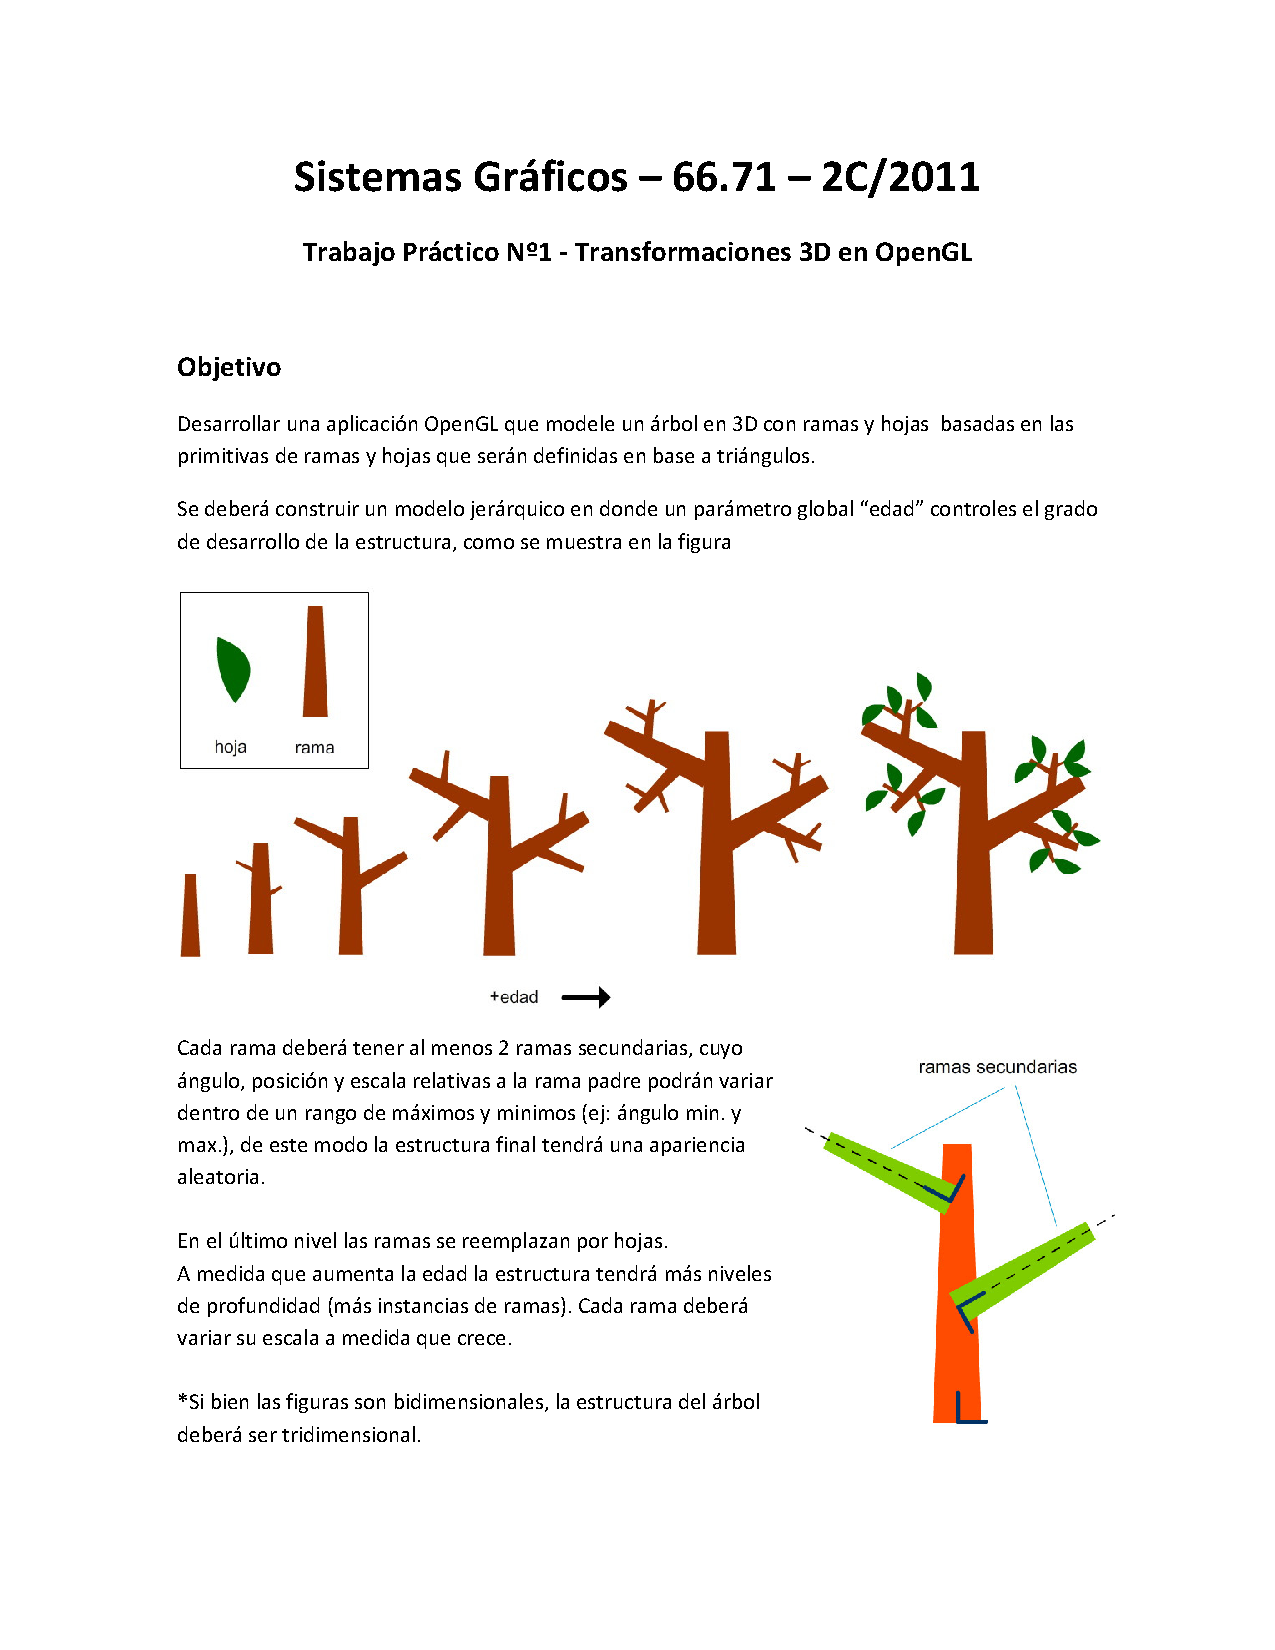
\includegraphics[trim = 25mm 30mm 10mm 35mm, clip,height=0.93\textheight,width=1.04\textwidth]{tp1-c2-2011.pdf}
\includegraphics[trim = 25mm 20mm 10mm 40mm, clip,height=0.95\textheight,width=1.04\textwidth,page={2}]{tp1-c2-2011.pdf}
\end{center}

\newpage


\section{Consideraciones de Dise\~no}
  Para la realizar el trabajo pr\'actico se tomaron en cuenta las siguientes consideraciones de dise\~no:
\begin{itemize}
 \item Se decidi\'o utilizar un algoritmo recursivo el cual en cada llamada dibuja un nivel del \'arbol.
 \item La altura de cada nivel del \'arbol depende en forma cuadr\'atica del nivel.
 \item La altura del \'arbol se actualiza aut\'omaticamente en funcion del tiempo de forma tal de producir la sensacion, mediante la animacion, 
de que el \'arbol va creciendo a medida que transcurre el mismo y alcanza su edad.
 \item El di\'ametro de cada tronco/rama depende de la altura de la misma.
 \item Para dibujar las hojas se utilizaron dos tri\'angulos empleando GL\_TRIANGLE\_STRIP de forma tal de que los mismos conformen un rombo.
 \item Para dibujar el tronco y las ramas se utilizaron  tri\'angulos para conformar un cono truncado junto con sus tapas.
 \item El rango de \'angulos de una rama respecto de su hija varia en funci\'on del nivel y en el rango: [40;40+NivelMaximo] [30 ; 30+NivelMaximo ]; correspondiendo
 el mayor \'angulo a las ramas ubicadas a menor altura en la rama padre.
 \item Despu\'es de cada nivel se realiza una rotaci\'on de 90 grados de forma tal de lograr repartir las ramas.
 \item Camara: La misma se puede hacer orbitar utilizando la tecla z Z, presionando la tecla c para capturar el movimiento del mouse y rotando la camara con el mismo
 . Tambi\'en permite acercarse utilizando la tecla + y alejarse utilizando la tecla -.
\end{itemize}



\section{Hip\'otesis}
Para realizar el trabajo pr\'actico se tomaron en cuenta las siguientes hip\'otesis:
\begin{itemize}
 \item Cada rama posee cuatro ramas hijas; o en su defecto cuatro hojas si se tratara del ante\'ultimo nivel.
 \item Por defecto el \'arbol tiene ocho niveles.
 \item 
\end{itemize}



\section{Compilaci\'on}
  Para compilar la aplicaci\'on bajo entornos Linux se provee un archivo de makefile.
  Para utilizar el mismo debe tenerse instalada la herramienta cmake. Para instalarla, por ejemplo, en una distribuci\'on Ubuntu se deben 
realizar los siguientes pasos: \\

1) sudo apt-get install cmake \\
2) Ingresar la contrase\~na de root del usuario. \\
3) Aceptar la descarga e instalaci\'on de los paquetes necesarios. \\ \\

Luego de instalada la herramienta, posicionados en el directorio donde se encuentra el trabajo pr\'actico es necesario crear un directorio build
de la siguiente forma: \\
mkdir build \\
cd build \\
cmake .. \\
make \\

Una vez realizados estos pasos, se dispondr\'a del ejecutable de nombre NOMBREEJECUTABLE.

\section{Ejecuci\'on}

Para ejecutar la aplicacio\'n bajo un entorno Linux se deben realizar los siguientes pasos: \\
1)Posicionarse en el directorio build creado anteriormente. \\
2)Ejecutar: \\
./NOMBREEJECUTABLE 


\section{Manual de Usuario}

 La aplicaci\'on permite realizar las siguientes acciones utilizando las teclas detalladas a continuacion:


Controles de teclado \\

R Reiniciar la animaci\'on de crecimiento \\
P Pausar/reanudar animaci\'on  \\
Q Incrementar velocidad de crecimiento  \\
A Decrementar velocidad de crecimiento  \\
q Salir de la aplicaci\'on  \\
a Muestra/esconde los ejes  \\
g Muestra/esconde la grilla  \\
c Captura/libera el mouse  \\
z Permite rotar alrededor del \'arbol en sentido antihorario  \\
Z Permite rotar alrededor del \'arbol en sentido horario  \\
+ Permite acercar la c\'amara al \'arbol  \\
- Permite alejar la c\'amara del \'arbol  \\



\end{document}

